\documentclass{article}

\usepackage{fontspec}
\defaultfontfeatures{Ligatures=TeX}
\usepackage{indentfirst}
\usepackage[brazilian]{babel}

\usepackage{graphicx}

\usepackage{textcomp}

%enconding
\usepackage[utf8]{inputenc}
\usepackage[T1]{fontenc}

\author{
  Pedro Correa\\
  \texttt{11718563} - \texttt{pedro.figueiredo563@al.faj.br}
}

\title{Lista de Execício}

\begin{document}

\maketitle

\newpage

\section{Identifique, utilizando a tabela acima, todos os tokens correspondentes ao programa abaixo. Cada linha da tabela será um token. (Linguagem PASCAL)}

\begin{center}
  \begin{tabular}{||p{0.7cm} p{3cm} p{3cm} p{3cm}||}
     \hline
     & Lexema & Classe & Padrão \\ [0.5ex]
     \hline\hline
     1 & int & palavra-chave & próprio lexema \\
     \hline
     2 & max & identificador & sequência de caracteres \\
     \hline
     3 & ( & pontuação & próprio lexema \\
     \hline
     4 & i & identificador & sequência de caracteres \\
     \hline
     5 & , & pontuação & próprio lexema \\
     \hline
     6 & j & identificador & sequência de caracteres \\
     \hline
     7 & ) & pontuação & próprio lexema \\
     \hline
     8 & int & palavra-chave & próprio lexema \\
     \hline
     9 & i & identificador & sequência de caracteres \\
     \hline
     10 & , & pontuação & próprio lexema \\
     \hline
     11 & j & identificador & sequência de caracteres \\
     \hline
     12 & ; & pontuação & próprio lexema \\
     \hline
     13 & /* retorna o maior dosinteiros entre i e j*/ & comentário & sequência de caracteresdelimitada por /* e */ \\
     \hline
     14 & \{ & delimitador escopo & próprio lexema \\
     \hline
     15 & return & palavra-chave & próprio lexema \\
     \hline
     16 & i & identificador & próprio \\
     \hline
     17 & > & operador relacional & próprio lexema \\
     \hline
     18 & j & identificador & próprio \\
     \hline
     19 & ? & operador ternário 1 & próprio lexema \\
     \hline
     20 & i & identificador & próprio \\
     \hline
     21 & ; & operador ternário 2 & próprio lexema \\
     \hline
     22 & j & identificador & próprio \\
     \hline
     23 & \} & delimitador escopo & próprio lexema \\
     \hline
  \end{tabular}
\end{center}

\section{Escreva expressões regulares para os conjuntos de caracteres a seguir e desenhe um diagrama de transições para cada expressão regular. Na sequência, escreva um algoritmo em linguagem de programação JAVA para cada diagrama de transição.}

\subsection{Cadeias de letras maiúsculas começando e terminando com a (minúsculo)}

\begin{figure}[h]
  \centering
    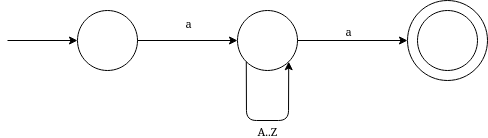
\includegraphics[scale=0.5]{./imgs/first.png}
\end{figure}

\subsection{Cadeias de dígitos que representam números pares.}

\begin{figure}[h]
  \centering
    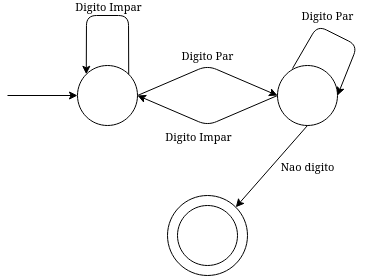
\includegraphics[scale=0.5]{./imgs/second.png}
\end{figure}

\newpage

\subsection{Cadeias de dígitos tais que todos os dígitos ímpares, se ocorrerem, ocorrem antes de todos os dígitos pares (se ocorrerem).}

\begin{figure}[h]
  \centering
    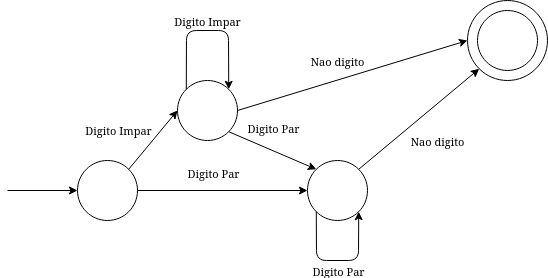
\includegraphics[scale=0.5]{./imgs/third.png}
\end{figure}

\subsection{Comentários, consistindo em uma cadeia cercada por /* e */, sem um */ intercalado}

\begin{figure}[h]
  \centering
    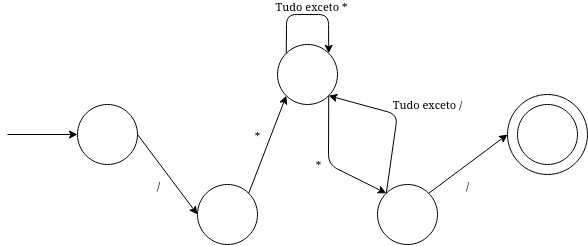
\includegraphics[scale=0.5]{./imgs/fourth.png}
\end{figure}

\end{document}

